\chapter{Informazione e cibernetica}

\section{Shannon}

Claude Shannon fu un matematico che lavorò per la Bell Labs.  Nel 1948 scrisse un articolo,
\fancyglitter{A Mathematical Theory of Communication}, in cui ha definito la teoria dell'informazione\footnote{Nella laurea magistrale è presente il corso "Teoria dell'Informazione" che approfondice questi argomenti.}: 
"il problema fondamentale della comunicazione è quello di 
riprodurre a un punto, esattamente o con qualche approssimazione, un messaggio
scelto in un altro punto".

\paragraph{Shannon definisce un contesto tecnico di termini:}
\begin{itemize}
    \item [$\Rightarrow$] \fancyglitter{Emittente - Ricevente}: il mittente è colui che invia il messaggio, il ricevente è colui che lo riceve.
    \item [$\Rightarrow$] \fancyglitter{Messaggio}: è l'informazione che si vuole trasmettere.
    \item [$\Rightarrow$] \fancyglitter{Rumore}: è tutto ciò che può interferire con la trasmissione del messaggio.
    \item [$\Rightarrow$] \fancyglitter{Informazione}: è la quantità di incertezza che si riduce nel ricevente dopo aver ricevuto il messaggio.
\end{itemize}


\nt{L'informazione in  sé è considerata in base al numero di possibili 
messaggi che possono essere inviati.}

\begin{figure}[h]
    \centering
    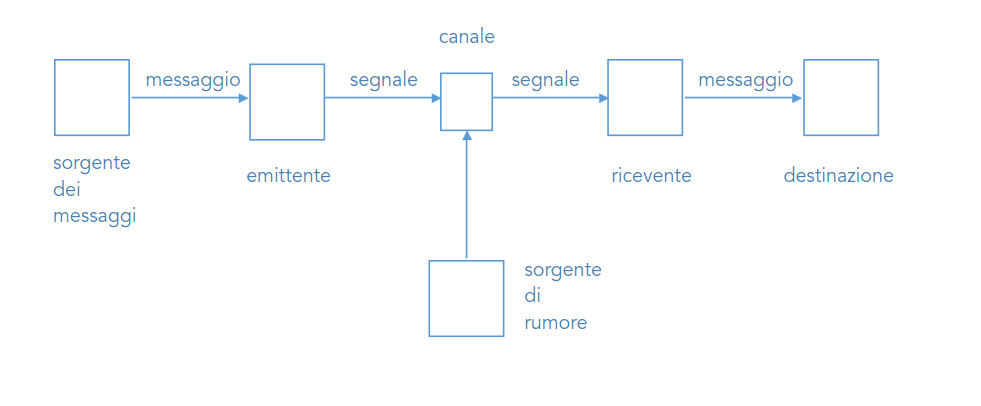
\includegraphics[scale=0.35]{images/Shannon.png}
    \caption{Schema di Shannon}
\end{figure}

\clm{}{}{
    L'informatica non è solamente uno scheletro che può essere riempito con
    qualsiasi cosa. Alla sua base vi sono idee e atteggiamenti fondanti che
    possono essere applicati in molti campi. Un esempio è la cibernetica che ha 
    avuto una breve durata (circa 20 anni), ma ha avuto un impatto molto forte
    in molte aree della scienza e della tecnologia.

    Esiste un'epistemologia dell'informatica, che ne studia
    le basi e le fondamenta. 
    
    Se si vuole approfondire l'argomento, nella prima parte del corso
    "Metodologie e Tecnologie Didattiche dell'Informatica" (MTDI o PREFIT)
    si ha una panoramica "motivazionale" sulle basi dell'informatica e sul suo
    essere una scienza.    
}

\subsection{Il modello di comunicazione}

Il modello di comunicazione di Shannon purtroppo non mette in evidenza
il fattore temporale e il ritardo. Quando si comunica in un contesto asincrono
bisogna utilizzare un sistema di feedback per capire se il messaggio è stato
ricevuto correttamente\footnote{Per esempio il sistema di ACK (Acknowledgement) di TCP
visto nel corso "Reti I"/"Reti di calcolatori".}. Il modello di comunicazione di Shannon
ha avuto varie interpretazioni, una delle quali è quella di Chapman.

\begin{figure}[h]
    \centering
    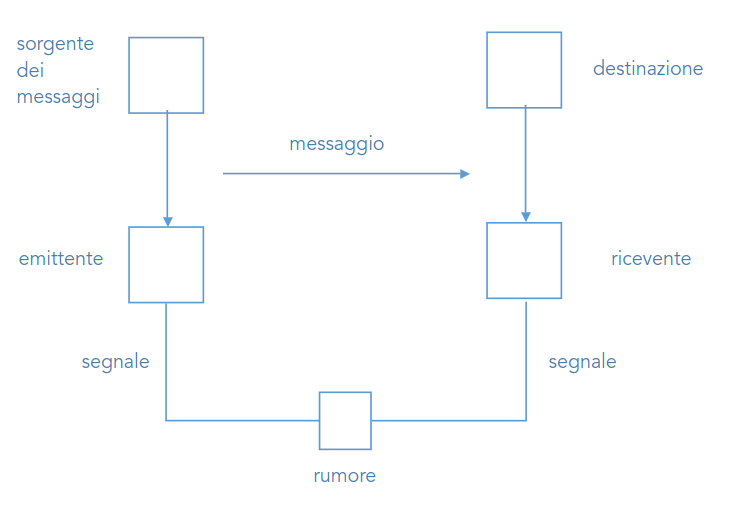
\includegraphics[scale=0.35]{images/Chapman.png}
    \caption{Modello di comunicazione di Shannon, reinterpretato da Chapman.}
\end{figure}

\paragraph{In questa interpretazione vengono identificati i livelli a cui i segnali possono esistere:}
\begin{itemize}
    \item [$\Rightarrow$] Nello strato basso è presente il rumore;
    \item [$\Rightarrow$] Al livello superiore è presente il messaggio.
\end{itemize}

\section{Nascita della cibernetica}

\subsection{Cibernetica e neurofisiologia}

La cibernetica viene codificata da Norbert Wiener nel 1948, e si occupa di studiare i sistemi di controllo e di comunicazione nei sistemi biologici 
e nelle macchine.
Von Neumann aveva come obiettivo l'unificazione del lavoro di McCulloch e Pitts con il lavoro di Shannon e di Turing. Per Wiener,
la nozione unificante era il feedback, mentre per von Neumann era la nozione di automa come
elaboratore di informazione.

\subsubsection{Lavori di von Neumann sugli automi:}

\begin{itemize}
    \item [$\Rightarrow$] \fancyglitter{The general and logical theory of automata}, Hixon Symposium, 1948;
    \item [$\Rightarrow$] \fancyglitter{Theory and organization of complicated automata}, serie di 5 lezioni all'università dello Illinois, 1949;
    \item [$\Rightarrow$] \fancyglitter{Probabilistic logics and the synthesis of reliable organisms from unreliable components}, appunti delle lezioni alla Caltech, 1952;
    \item [$\Rightarrow$] \fancyglitter{The Theory of Automata: Construction, Reproduction, Homogeneity}, 1952-1953;
    \item [$\Rightarrow$] \fancyglitter{The computer and the brain}, Yale University Press, 1956 pubblicato postumo.
\end{itemize}

\subsubsection{}

\paragraph{Per ricapitolare le relazioni tra i vari "attori":}

\begin{itemize}
    \item [$\Rightarrow$] \fancyglitter{Shannon - Turing}: si incontrano nel 1943 ai Bell Labs, e discutono di comunicazione\footnote{Da ricordare Enigma e la crittografia.};
    \item [$\Rightarrow$] \fancyglitter{Wiener - Von Neumann - McCulloch - Pitts}: partecipano alle conferenze di Macy la cui nozione centrale è il messaggio (con le accezioni di Shannon);
    \item [$\Rightarrow$] \fancyglitter{Wiener - McCulloch - Pitts}: membri del RLE;
    \item [$\Rightarrow$] \fancyglitter{Von Neumann - Turing}: si incontrano nel 1937 a Princeton. Nel 1939 von Neumann offre a Turing un posto di lavoro come assistente a Princeton, ma Turing rifiuta;
    \item [$\Rightarrow$] \fancyglitter{Shannon - Wiener}: sviluppano una teoria matematica e della comunicazione basata sulla concezione dell'informazione/entropia di un insieme di messaggi.
\end{itemize}

\clm{}{}{Pare che Shannon adorasse il monociclo e che spesso tenesse dei party
in cui si esibiva in numeri di equilibrismo.
}

\begin{figure}[h]
    \centering
    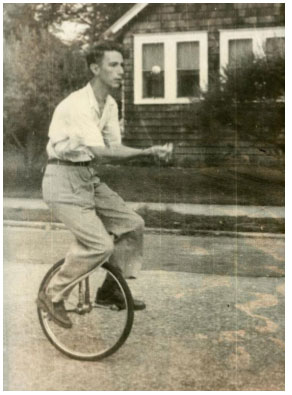
\includegraphics[scale=0.30]{images/Shannon monocycle.jpg}
    \caption{Shannon sul monociclo}
\end{figure}

\subsection{Von Neumann e la termodinamica del calcolo}

Von Neumann cercò di valutare il costo energetico minimo per un
atto elementare di generazione di informazioni. Da ciò deriva, nel 1949,
la formula:

$$kT \log_e N$$

\begin{itemize}
    \item [$\Rightarrow$] $k$: costante di Boltzmann;
    \item [$\Rightarrow$] $T$: temperatura;
    \item [$\Rightarrow$] $N$: numero di alternative o possibili stati.
\end{itemize}
\subsubsection{}
Questo calcolo attirò le attenzioni di \fancyglitter{Landauer}, un fisico teorico, 
che non riuscì a dimostrarlo, ma osservò che le operazioni logicamente
irreversibili (come l'operazione di cancellazione di un bit) generano entropia
pari alla quantità di informazione cancellata. \fancyglitter{Bennet}, un suo studente,
nel 1973, dimostrò che ogni calcolo può essere reso logicamente reversibile.
\fancyglitter{Fredkin}, un altro fisico teorico, 
lavorò a una base fisica per i calcoli reversibili.

\nt{Da questo tipo di interessi nasce la computazione quantistica (
    che cosa succede se si considera la computazione come composta da operazioni
    meccaniche?).}

\begin{figure}[h]
    \centering
    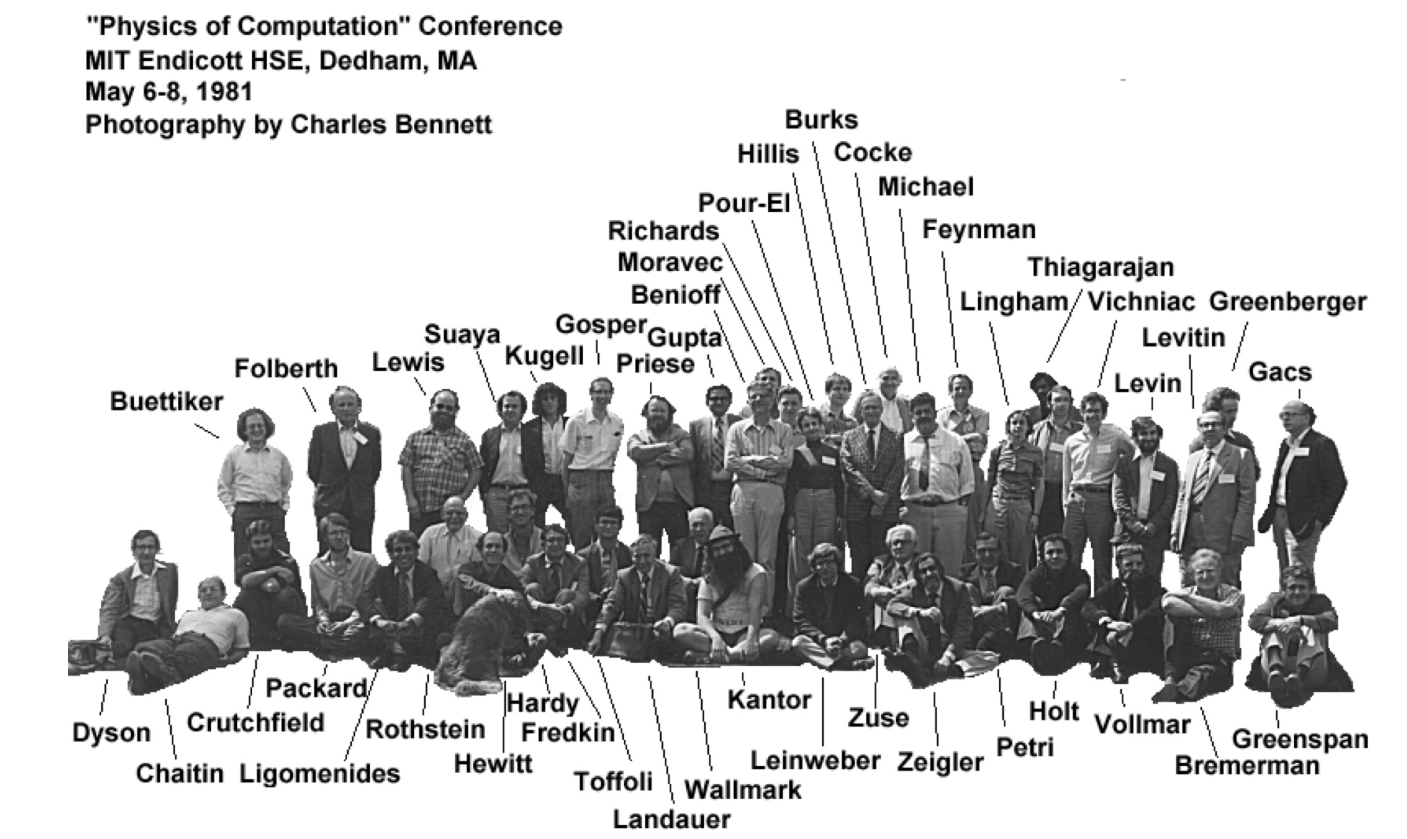
\includegraphics[scale=0.3]{images/Comp.png}
    \caption{Physics of Computation}
\end{figure}

\clm{}{}{
    \begin{itemize}
        \item [$\Rightarrow$] \fancyglitter{Bennet}: è un fisico teorico, non è direttamente
        presente nella foto perché fu lui a scattarla;
        \item [$\Rightarrow$] \fancyglitter{Landauer}: è presente nella foto in primo piano;
        \item [$\Rightarrow$] \fancyglitter{Fredkin}: è presente nella foto, vicino a Landauer e Toffoli;
        \item  [$\Rightarrow$] \fancyglitter{Toffoli}: fu uno studioso di fisica della computazione che interagi con
        Burks;
        \item  [$\Rightarrow$] \fancyglitter{Burks}: in secondo piano;
        \item [$\Rightarrow$] \fancyglitter{Feynman}, \fancyglitter{Dysan} e altri fisici famosi;
        \item [$\Rightarrow$] \fancyglitter{Zuse}: già visto nella prima parte del corso, inventore dello Z1;
        \item [$\Rightarrow$] \fancyglitter{Kantor}: inventore e specialista dell'informazione come principio ontologico;
        \item [$\Rightarrow$] \fancyglitter{Holt}: esperto di cibernetica;
        \item [$\Rightarrow$] \fancyglitter{Gosper}: inventore della configurazione ad aliante, uno dei primi "hacker".
    \end{itemize}
}

\section{La cibernetica}

Quando si \fancyglitter{comunica} con un'altra persona le si trasmette un
messaggio, e quando l'altra persona risponde, si riceve un messaggio che contiene
informazioni accessibili a sé stessi e all'altro. Ma anche quando si \fancyglitter{controllano}
le azioni di un'altra persona le si comunica un messaggio (in forma imperativa). 
Tutto ciò si riduce a uno \fancyglitter{scambio di messaggi}.

\dfn{Cibernetica}{
    La \newfancyglitter{cibernetica} può essere vista come una teoria della
    trasmissione dei messaggi e delle sue condizioni che presentano un successo.
}

\nt{Il computer diventa un oggetto cibernetico, in quanto è inserito in un
contesto di comunicazione con esseri umani o con altri computer.}

\subsection{Il feedback e il flusso di messaggi}
\label{feedback}
Wiener confrontava l'attività umana con quella di figure che danzano sopra
un carillon secondo un modello. Tuttavia il modello in esame è un modello
predisposto in cui il loro passato non ha influenza sul loro futuro. Non 
c'è feedback.

\begin{figure}[h]
    \centering
    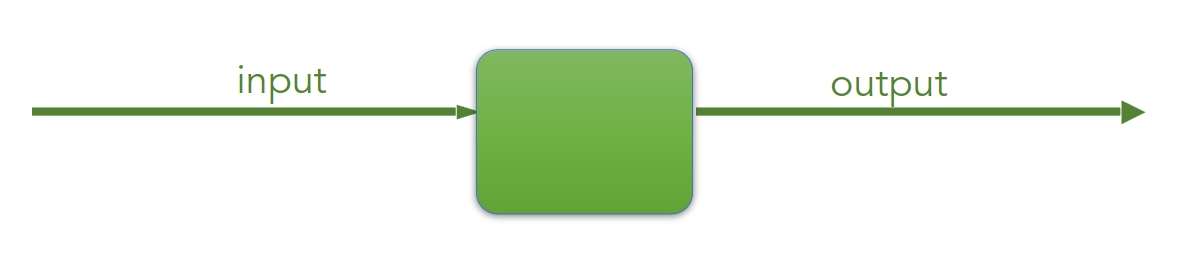
\includegraphics[scale=0.35]{images/IO.png}
    \caption{Modello IO}
\end{figure}

\subsubsection{}

Holt propose l'idea che quando una persona scrive su una macchina premendo il tasto
esso fornisce un feedback tornando indietro. La temporizzazione dei tasti è
ciò che consente la scrittura.
Questo si può estendere all'utente e all'interfaccia: la scelta di un'interfaccia comporta
la progettazione dell'utente indicando cosa si può o non si può fare.

\ex{Scatola nera}{
    Si immagini una scatola con dei pulsanti che si possono premere. Quando si preme un pulsante
    si accende una luce. Prima di poter schiacciare un altro pulsante bisogna controllare che la luce
    si sia accesa. In questo caso la luce è il feedback.
    \begin{center}
        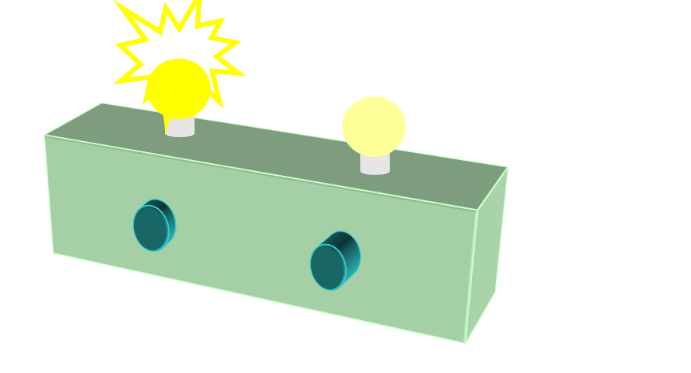
\includegraphics[scale=0.35]{images/Scatola nera.png}
    \end{center}

    Se i pulsanti sono premuti da un operatore che non può vedere le luci e 
    le luci sono visibili a un altro operatore che non può premere i pulsanti,
    non si potrebbe stabilire una corrispondenza tra luci e pulsanti e dunque la connessione non ha 
    succeso.

    \begin{center}
        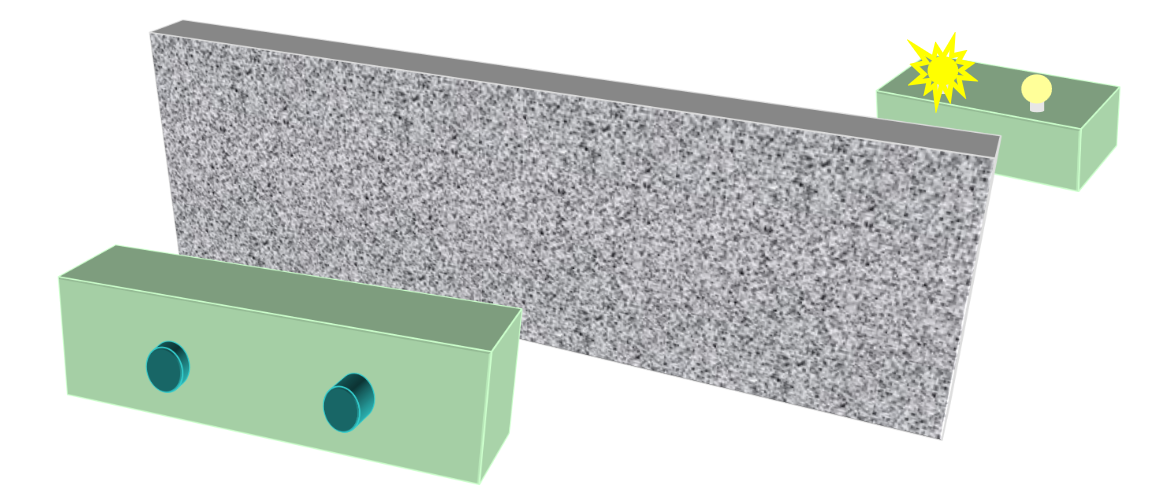
\includegraphics[scale=0.35]{images/Scatola nera 2.png}
    \end{center}

}

\subsection{Osservatori}

In alcuni sistemi, per esempio un termostato, è l'osservatore a concettualizzare il ciclo.
Nei sistemi di secondo ordine, l'osservatore è esso stesso parte del sistema osservato.

\begin{figure}[h]
    \centering
    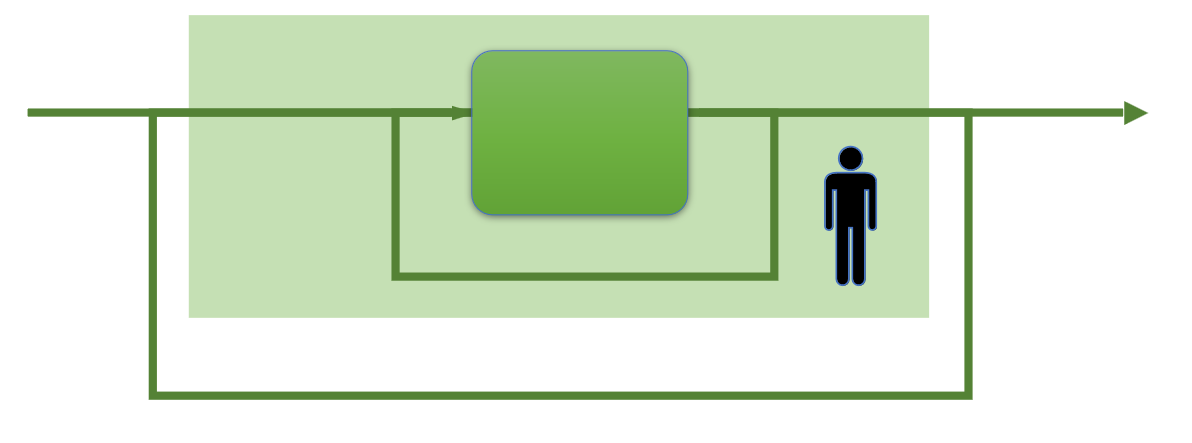
\includegraphics[scale=0.25]{images/Osservatore.png}
    \caption{Osservatore}
\end{figure}

\subsection{Comunicazione sincrona e asincrona}

\dfn{Comunicazione sincrona}{
    La \newfancyglitter{comunicazione sincrona} è una comunicazione in cui il mittente e il ricevente
    sono sincronizzati. 
    
    In una comunicazione sincrona è presente un unico sistema di riferimento
    temporale condiviso da tutti i partecipanti. 

}

\ex{Comunicazione sincrona}{
    \begin{itemize}
        \item [$\Rightarrow$] Chiamata telefonica;
        \item [$\Rightarrow$] Conversazione faccia a faccia;
        \item [$\Rightarrow$] Sistema di posta elettronica in cui i messaggi impiegano $n$ secondi per 
        essere consegnati;
        \item [$\Rightarrow$] Segnali di fumo.
    \end{itemize}
}

\dfn{Comunicazione asincrona}{
    La \newfancyglitter{comunicazione asincrona} è una comunicazione in cui il mittente e il ricevente
    non sono sincronizzati. 
    
    In una comunicazione asincrona non è presente un unico sistema di riferimento
    temporale condiviso da tutti i partecipanti. 

}

\ex{Comunicazione asincrona}{
    \begin{itemize}
        \item [$\Rightarrow$] Sistema di posta elettronica con garanzia di consegna entro $n$ secondi;
        \item [$\Rightarrow$] Sistema postale ordinario;
        \item [$\Rightarrow$] Messaggi in bottiglia.
    \end{itemize}
}

\nt{Nella comunicazione asincrona è necessario un sistema di feedback per capire se il messaggio è stato ricevuto.}

\dfn{Circuiti asincroni}{
    I \newfancyglitter{circuiti asincroni} sono circuiti in cui i segnali di controllo
    non sono sincronizzati con un segnale di clock (orologio globale).
}

\cor{C-Muller}{
    Un elemento asincrono è il C-Muller per cui l'uscita è 1 se e solo se
    entrambi gli ingressi sono 1 e diventa 0 se entrambi gli ingressi sono 0.
}

\begin{figure}[h]
    \centering
    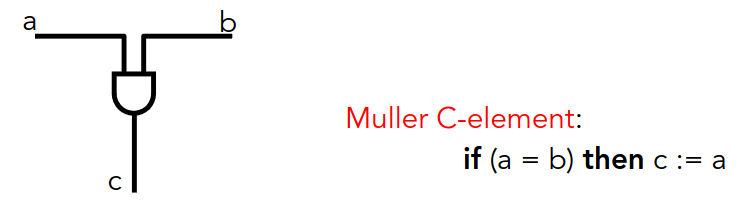
\includegraphics[scale=0.33]{images/C-Muller.png}
    \caption{C-Muller}  
\end{figure}

\nt{Combinando più C-Muller si può costruire un circuito asincrono che implementa
le micropipeline.}

\begin{figure}[h]
    \centering
    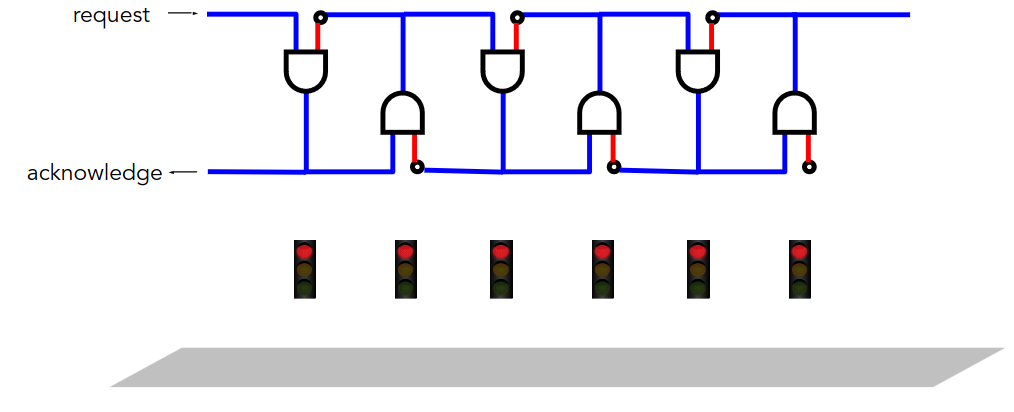
\includegraphics[scale=0.25]{images/Micropipeline.png}
    \caption{Micropipeline}
\end{figure}

\cor{Reti di Petri}{
    Grafi che generalizzano gli automi a stati finiti (DFA e NFA).
    Si hanno posti (condizioni) e transizioni (eventi).
}

\begin{figure}[h]
    \centering
    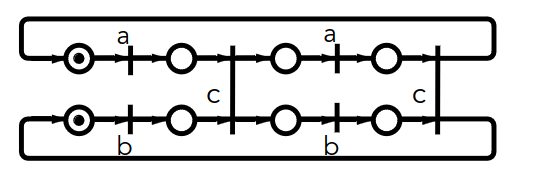
\includegraphics[scale=0.35]{images/Petri.png}
    \caption{Rete di Petri}
\end{figure}










